\section{方法}
\label{sec:method}

\subsection{系统概览}
\label{sec:overview}

系统由三个阶段组成，如图~\ref{fig:pipeline} 所示。第一阶段接收文档与元数据；第二阶段
用分类器给出主题标签与置信度，并用声明抽取器给出支持该标签的原文片段；第三阶段把
低置信度或证据不足的条目转交人工审阅。审阅者可以接受、修改或拒绝模型的提议，所有
动作写入审计记录。

\begin{figure}[htbp]
  \centering
  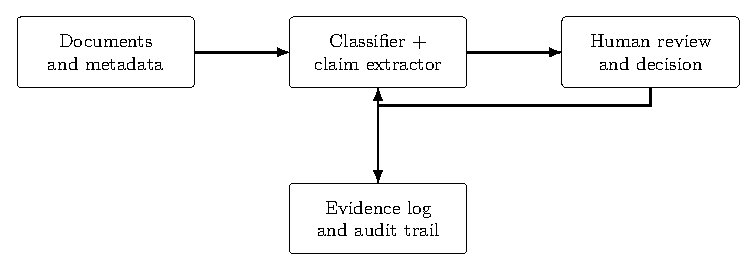
\includegraphics[width=0.86\textwidth]{figures/example-figure.pdf}
  \caption{人机协同文档分流的三阶段流程。低置信度条目进入人工审阅，审阅动作与证据写入审计记录。}
  \label{fig:pipeline}
  \figsource{作者自绘；人机分工见第~\ref{sec:division} 节。}
\end{figure}

\subsection{数据与人机分工}
\label{sec:division}

评估使用一个小型合成语料库：48 份文档，覆盖两个主题，每份文档带有一个人工标注的
主题标签。语料库不包含真实学生、合作方或个人信息；这是评估可公开的前提，也是本原型
的边界。

人机分工遵循「模型提议、人来决定」的原则。模型只输出标签、置信度与证据片段，不自动
拒绝文档；置信度低于 0.8 或证据片段为空时，条目必须进入人工审阅。审阅者的最终标签
是唯一写入正式记录的标签，模型输出只作为建议保留。
